\documentclass{report}

\usepackage[utf8]{inputenc}
\usepackage[T1]{fontenc}      
\usepackage[francais]{babel}
\usepackage{graphicx}
\usepackage{circuitikz}
\usepackage[squaren, Gray]{SIunits}
\usepackage{sistyle}
\usepackage[autolanguage]{numprint}
\usepackage{pgfplots}
\usepackage{geometry}
\usepackage{hyperref}
\usepackage{caption}
\usepackage{amsmath,amssymb,array}
\usepackage{url}
\usepackage{fancyhdr}
\usepackage{layout}
\usepackage[version=3]{mhchem}
\usepackage{array} 
\newcommand{\reporttitle}{Synthèse de l’ammoniac}     % Titre
\newcommand{\reportauthor}{Corentin \bsc{Joachim} \\ Xavier \bsc{Lambein} \\Edward \bsc{Nicol}\\ Léa \bsc{Paulus}\\ Abbas \bsc{Sliti}} % Auteur
\newcommand{\reportsubject}{Projet Q3} % Sujet
\newcommand{\HRule}{\rule{\linewidth}{0.5mm}}
\newcommand{\copyrigh}{{\tiny \textregistered}}
\setlength{\parskip}{1ex} % Espace entre les paragraphes

\hypersetup{
    pdftitle={\reporttitle},%
     pdfauthor={\reportauthor},%
    pdfsubject={\reportsubject},%
    pdfkeywords={rapport} {vos} {mots} {clés}
}


\setlength{\headheight}{12pt}
\setlength{\headsep}{12pt}

\pagestyle{fancy}
\lhead{\leftmark{}}
\rhead{P3 - 2014 - gr54}
\cfoot{\thepage{}}
\begin{document}
\begin{titlepage}

\begin{center}

% Upper part of the page

\textsc{\Large Université Catholique de Louvain}\\[0.5cm]

\textsc{\LARGE Rapport de projet du troisième quadrimestre}\\[0.2cm]
\textsc{\LARGE LFSAB1503}\\[0.2cm]

% Title
\HRule \\[0.2cm]
{\huge \bfseries Synthèse de l'ammoniac}\\
\HRule \\[0.2cm]

% Author and supervisor
\begin{center}
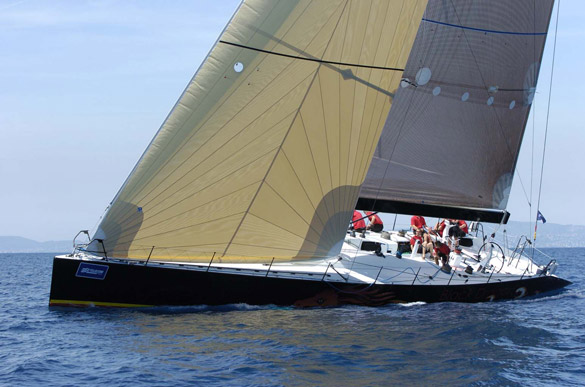
\includegraphics[trim=0cm 2cm 0cm 2cm, clip, width=15cm]{Shema/kevlar_taffeta2.jpg}
\end{center}
\HRule \\[0 cm]
%inventer un petit texte cool :)
Dans le cadre de notre projet Q3, il nous a été demandé d'analyser et de proposer des pistes d'amélioration pour le procédé Haber-Bosch. En effet, la synthèse d'ammoniac rejette énormément de \ce{CO2}, c'est pourquoi nous avons exploré des solutions plus écologiques telles que le biométhane, l'hydrolyse ou encore des algues produisant de l'\ce{H2}.
\HRule \\[0.2cm]

\begin{minipage}{0.4\textwidth}
\begin{flushleft} \large
\emph{Auteurs:}
Corentin \bsc{Joachim} \\ Xavier \bsc{Lambein} \\Edward \bsc{Nicol}\\ Léa \bsc{Paulus}\\ Abbas \bsc{Sliti}
\end{flushleft}
\end{minipage}
\begin{minipage}{0.4\textwidth}
\begin{flushright} \large
\emph{Cours:} \\
FSAB1503\\
\emph{Groupe:} \\
1254\\
\emph{Tuteur:} \\
Vincent Destoop \textsc{}
\end{flushright}
\end{minipage}
\vspace{0.4cm}
% Bottom of the page

\begin{minipage}{0.3\textwidth}
\begin{flushleft}

\includegraphics[height=2cm]{Shema/logo_UCL_NEW_janv2013.JPG}
\end{flushleft}
\end{minipage}
\begin{minipage}{0.3\textwidth}
\begin{center}
{\large FSA12BA}\\
{\large \today}
\end{center}
\end{minipage}
\begin{minipage}{0.3\textwidth}
\begin{flushright}

\includegraphics[height=1cm]{Shema/epl-logo.jpg}
\end{flushright}
\end{minipage}
\end{center}
\end{titlepage}
\tableofcontents


%don"t write in this one ! :)
%thibaut's part
%Adrien's part
%coco's part
%Geo's part
%Léa's part
\end{document}